\begin{frame}
	\frametitle{Custo M\'edio e Lucro}
	Em geral:
	\begin{align*}
		\text{Lucro} &= \text{Receita Total} - \text{Custo Total}\\
		\Pi &= RT - CT \\
		\Pi &= PQ-CF-CV \\
		\Pi &= Q(P-CTM) = Q(P-CVM-CFM)
	\end{align*}

	Se o pre\c co unit\'ario de venda do bem for suficientemente grande, $P>CTM$, a empresa ter\'a lucro, caso contr\'ario, ter\'a prejuizo.
\end{frame}

\begin{frame}
	\frametitle{Equil\'ibrio no Mercado Competitivo (curto prazo)}
	\begin{itemize}
		\item O mercado est\'a em equil\'ibrio quando se atinge um pre\c co e uma quantidade tais que os consumidores e os produtores n\~ao querem alterar as suas escolhas individuais...\pause
		\item Os consumidores compram exactamente a quantidade que estavam dispostos a adquirir\pause
		\item Os produtores vendem exactamente a quantidade que planificavam oferecer\pause
		\item Ao pre\c co de equil\'ibrio, a quantidade procurada \'e igual \`a quantidade oferecida
	\end{itemize}
\end{frame}

\begin{frame}
	\frametitle{Equil\'ibrio de Mercado}
	\begin{center}
		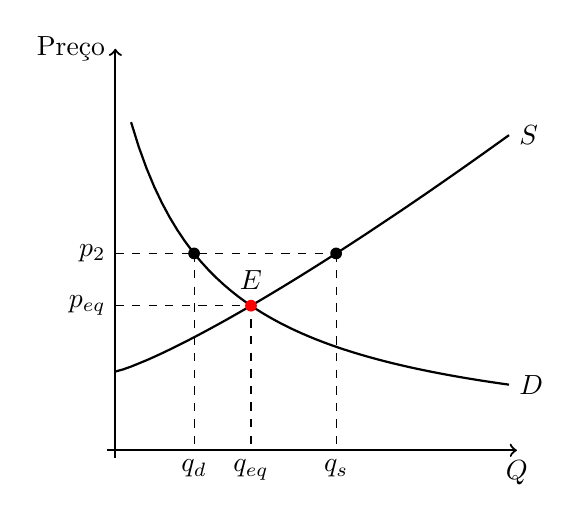
\begin{tikzpicture}[
			scale = 1,
			every node/.style = {scale = 1},
			declare function = {
				s(\x) = 1+(\x/2)^(3/2.5);
				d(\x) = 5/(\x+1);
			}
			]

			\draw[thick,->] (-0.1,0) -- (5.1,0)node[below]{$Q$};
			\draw[thick,->] (0,-0.1) -- (0,5.1)node[left]{Pre\c co};

			\onslide<2->{
				\draw[thick,samples=50,domain=0.2:5,variable=\x] plot (\x,{d(\x)})node[right]{$D$};
			}

			\onslide<3->{
				\draw[thick,samples=50,domain=0:5,variable=\x] plot (\x,{s(\x)})node[right]{$S$};
			}
				
			\def\ea{1}
			\def\eb{2.80397}
			\def\eq{1.72301}

			\onslide<4>{
				\draw(\ea,{d(\ea)}) node[circle,fill,inner sep=1.5]{};
			}

			\only<4>{
				\draw(\eb,{s(\eb)}) node[circle,fill,inner sep=1.5]{};
				\draw[dashed](0,{s(\eb)})node[left]{$p_2$} -- (\eb,{s(\eb)});
				\draw[dashed](\ea,{d(\ea)}) -- (\ea,0)node[below]{$q_d$};
				\draw[dashed](\eb,{s(\eb)}) -- (\eb,0)node[below]{$q_s$};
			}

			\onslide<5->{
				\draw[dashed] (0,{d(\eq)})node[left]{$p_{eq}$} -- (\eq,{d(\eq)}) -- (\eq,0)node[below]{$q_{eq}$};
				\draw(\eq,{d(\eq)}) node[black,circle,fill=red,inner sep=1.5,label=above:{$E$}]{};
			}
			
		\end{tikzpicture}
	\end{center}
\end{frame}

\begin{frame}
	\frametitle{Equil\'ibrio de Mercado}
	\begin{itemize}
		\item O equil\'ibrio surge pelo ajustamento autom\'atico de pre\c co, processo que Adam Smith (1776) baptizou como ``A M\~ao Invis\'ivel,'' desde que os agentes econ\'omicos sejam racionais e, portanto, escolham de forma \'optima
		\item Nos mercados concorrenciais, n\~ao havendo falhas de mercado, este equil\'ibrio \'e eficiente!
	\end{itemize}
\end{frame}

\begin{frame}
	\frametitle{Excesso de Oferta: o pre\c co desce}
	\begin{center}
		\begin{tikzpicture}[
			scale = 1,
			every node/.style = {scale = 0.8},
			declare function = {
				s(\x) = 1+(\x/2)^(3/2.5);
				d(\x) = 5/(\x+1);
			}
			]

			\draw[thick,->] (-0.1,0) -- (5.1,0)node[below]{$Q$};
			\draw[thick,->] (0,-0.1) -- (0,5.1)node[left]{Pre\c co};

			\draw[thick,samples=50,domain=0.2:5,variable=\x] plot (\x,{d(\x)})node[right]{$D$};
			\draw[thick,samples=50,domain=0:5,variable=\x] plot (\x,{s(\x)})node[right]{$S$};
				
			\def\ea{1}
			\def\eb{2.80397}
			\def\eq{1.72301}

			\draw(\ea,{d(\ea)}) node[circle,fill,inner sep=1.5]{};

			\draw(\eb,{s(\eb)}) node[circle,fill,inner sep=1.5]{};
			\draw[draw=none](0,{s(\eb)})node[left]{$p_1$} -- (\eb,{s(\eb)});
			\draw[dashed](\ea,{d(\ea)}) -- (\ea,0)node[below]{$q_d$};
			\draw[dashed](\eb,{s(\eb)}) -- (\eb,0)node[below]{$q_s$};

			\draw[dashed] (0,{d(\eq)})node[left]{$p_{eq}$} -- (\eq,{d(\eq)}) -- (\eq,0)node[below]{$q_{eq}$};
			\draw[pen colour={red},ultra thick,decorate,decoration={calligraphic brace},yshift=0.2cm] (\ea,{d(\ea)}) -- (\eb,{s(\eb)}) node[midway,above=10pt]{Excesso de Oferta};

			\draw(\eq,{d(\eq)}) node[black,circle,fill=red,inner sep=1.5]{};

			\onslide<2>{
				\draw[ultra thick, red, ->] (\eq,{d(\ea)}) -- (\eq,{d(\eq)+0.1});
			}
			
		\end{tikzpicture}
	\end{center}
	\[p=p_1 \ \Rightarrow \ q_s>q_d\]
\end{frame}

\begin{frame}
	\frametitle{Excesso de Procura: o pre\c co sobe}
	\begin{center}
		\begin{tikzpicture}[
			scale = 1,
			every node/.style = {scale = 0.8},
			declare function = {
				s(\x) = 1+(\x/2)^(3/2.5);
				d(\x) = 5/(\x+1);
			}
			]

			\draw[thick,->] (-0.1,0) -- (5.1,0)node[below]{$Q$};
			\draw[thick,->] (0,-0.1) -- (0,5.1)node[left]{Pre\c co};

			\draw[thick,samples=50,domain=0.2:5,variable=\x] plot (\x,{d(\x)})node[right]{$D$};
			\draw[thick,samples=50,domain=0:5,variable=\x] plot (\x,{s(\x)})node[right]{$S$};
				
			\def\ea{0.75}
			\def\eb{2.80397}
			\def\eq{1.72301}

			\draw(\ea,{s(\ea)}) node[circle,fill,inner sep=1.5]{};

			\draw(\eb,{d(\eb)}) node[circle,fill,inner sep=1.5]{};
			\draw[draw=none](0,{s(\ea)})node[left]{$p_2$} -- (\eb,{d(\eb)});
			\draw[dashed](\ea,{s(\ea)}) -- (\ea,0)node[below]{$q_s$};
			\draw[dashed](\eb,{d(\eb)}) -- (\eb,0)node[below]{$q_d$};

			\draw[dashed] (0,{d(\eq)})node[left]{$p_{eq}$} -- (\eq,{d(\eq)}) -- (\eq,0)node[below]{$q_{eq}$};
			\draw[pen colour={red},ultra thick,decorate,decoration={calligraphic brace,mirror},yshift=-0.2cm] (\ea,{s(\ea)}) -- (\eb,{d(\eb)}) node[midway,below=5pt]{Excesso de Procura};

			\draw(\eq,{s(\eq)}) node[black,circle,fill=red,inner sep=1.5]{};

			\onslide<2>{
				\draw[ultra thick, red, ->] (\eq,{s(\ea)}) -- (\eq,{s(\eq)-0.1});
			}
			
		\end{tikzpicture}
	\end{center}
	\[p=p_2 \ \Rightarrow \ q_s<q_d\]
\end{frame}

\begin{frame}
	\frametitle{Altera\c c\~oes ao Equil\'ibrio: Expans\~ao de Procura}
	\begin{center}
		\begin{tikzpicture}[
			scale = 1,
			every node/.style = {scale = 0.8},
			declare function = {
				s(\x) = 1+(\x/2)^(3/2.5);
				d(\x) = 5/(\x+1);
				d2(\x) = d(\x-0.5)+0.5;
			}
			]

			\def\ea{0.75}
			\def\eb{2.80397}
			\def\eq{1.72301}
			\def\noeq{3.2419455}
			\def\neweq{2.38325}

			\draw[thick,->] (-0.1,0) -- (5.1,0)node[below]{$Q$};
			\draw[thick,->] (0,-0.1) -- (0,5.1)node[left]{Pre\c co};

			\draw[thick,samples=50,domain=0:5,variable=\x] plot (\x,{s(\x)})node[right]{$S$};

			\onslide<1-2>{
				\draw[dashed] (0,{d(\eq)})node[left]{$p_{eq}$} -- (\eq,{d(\eq)}) -- (\eq,0)node[below]{$q_{eq}$};
			}

			\onslide<1-3>{
				\draw[thick,samples=50,domain=0.2:5,variable=\x] plot (\x,{d(\x)})node[right]{$D$};
			}

			\onslide<2->{
				\draw[thick,red,samples=50,domain=0.7:5,variable=\x] plot (\x,{d2(\x)})node[right]{$D'$};
			}

			\onslide<3->{
				\draw[dashed] (0,{d(\eq)})node[left]{$p_{0}$} -- (\eq,{d(\eq)}) -- (\eq,0)node[below]{$q_{s}$};
				\draw[dashed] (0,{d(\eq)}) -- (\noeq,{d2(\noeq)}) -- (\noeq,0)node[below]{$q_{d'}$};
			}

			\onslide<4->{
				\draw[pen colour={red},ultra thick,decorate,decoration={calligraphic brace,mirror},yshift=-0.2cm] (\eq,{s(\eq)}) -- (\noeq,{d2(\noeq)}) node[midway,below=5pt]{Excesso de Procura};
			}
			
			\onslide<5>{
				\draw[ultra thick, red, ->] (\neweq,{s(\eq)}) -- (\neweq,{s(\neweq)-0.1});
			}

		\end{tikzpicture}
	\end{center}
\end{frame}

\begin{frame}
	\frametitle{Altera\c c\~oes ao Equil\'ibrio: Expans\~ao de Oferta}
	\begin{center}
		\begin{tikzpicture}[
			scale = 1,
			every node/.style = {scale = 0.8},
			declare function = {
				s(\x) = 1+(\x/2)^(3/2.5);
				s2(\x) = s(\x-0.5)-0.5;
				d(\x) = 5/(\x+1);
				d2(\x) = d(\x-0.5)+0.5;
			}
			]

			\def\ea{0.75}
			\def\eb{2.80397}
			\def\eq{1.72301}
			\def\noeq{3.04638}
			\def\neweq{2.42959}

			\draw[thick,->] (-0.1,0) -- (5.1,0)node[below]{$Q$};
			\draw[thick,->] (0,-0.1) -- (0,5.1)node[left]{Pre\c co};

			\draw[thick,samples=50,domain=0.2:5,variable=\x] plot (\x,{d(\x)})node[right]{$D$};;

			\onslide<1-2>{
				\draw[dashed] (0,{d(\eq)})node[left]{$p_{eq}$} -- (\eq,{d(\eq)}) -- (\eq,0)node[below]{$q_{eq}$};
			}

			\onslide<1-3>{
				\draw[thick,samples=50,domain=0:5,variable=\x] plot (\x,{s(\x)})node[right]{$S$};
			}

			\onslide<2->{
				\draw[thick,red,samples=50,domain=0.7:5,variable=\x] plot (\x,{s2(\x)})node[right]{$S'$};
			}

			\onslide<3->{
				\draw[dashed] (0,{d(\eq)})node[left]{$p_{0}$} -- (\eq,{d(\eq)}) -- (\eq,0)node[below]{$q_{d}$};
				\draw[dashed] (0,{d(\eq)}) -- (\noeq,{s2(\noeq)}) -- (\noeq,0)node[below]{$q_{s'}$};
			}

			\onslide<4->{
			\draw[pen colour={red},ultra thick,decorate,decoration={calligraphic brace},yshift=0.2cm] (\eq,{d(\eq)}) -- (\noeq,{s2(\noeq)}) node[midway,above=10pt]{Excesso de Oferta};
			}
			
			\onslide<5>{
				\draw[ultra thick, red, ->] (\neweq,{s(\eq)}) -- (\neweq,{s2(\neweq)+0.1});
			}

		\end{tikzpicture}
	\end{center}
\end{frame}

\begin{frame}
	\frametitle{Expans\~ao da Procura/Oferta}
	\begin{center}
		{
		\renewcommand{\arraystretch}{2}
		\begin{tabular}{|c|cc|}
			\hline
			& Q & P \\
			\hline \hline
			$\uparrow$ Procura & $\uparrow$ & $\uparrow$ \\
			$\uparrow$ Oferta & $\uparrow$ & $\downarrow$ \\
			$\uparrow$ Procura e $\uparrow$ Oferta & $\uparrow$ & ? \\
			\hline
		\end{tabular}
		}
	\end{center}
\end{frame}

\begin{frame}
	\frametitle{Altera\c c\~oes ao Equil\'ibrio: Expans\~ao de Oferta}
	\begin{center}
		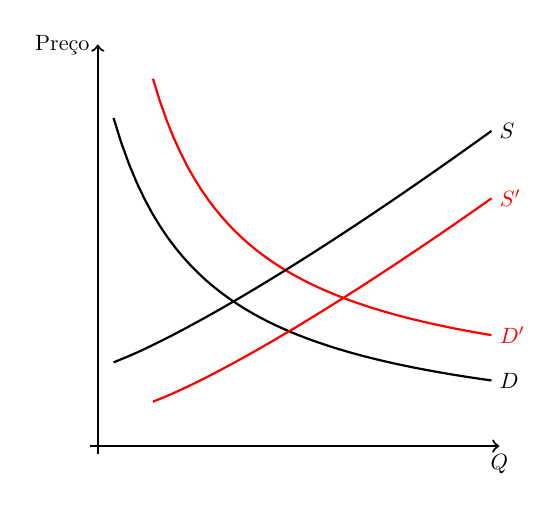
\begin{tikzpicture}[
			scale = 1,
			every node/.style = {scale = 0.8},
			declare function = {
				s(\x) = 1+(\x/2)^(3/2.5);
				s2(\x) = s(\x-0.5)-0.5;
				d(\x) = 5/(\x+1);
				d2(\x) = d(\x-0.5)+0.5;
			}
			]

			\def\ea{0.75}
			\def\eb{2.80397}
			\def\eq{1.72301}
			\def\noeq{3.04638}
			\def\neweq{2.42959}

			\draw[thick,->] (-0.1,0) -- (5.1,0)node[below]{$Q$};
			\draw[thick,->] (0,-0.1) -- (0,5.1)node[left]{Pre\c co};

			\draw[thick,samples=50,domain=0.2:5,variable=\x] plot (\x,{d(\x)})node[right]{$D$};
			\draw[red,thick,samples=50,domain=0.7:5,variable=\x] plot (\x,{d2(\x)})node[right]{$D'$};
			\draw[thick,samples=50,domain=0.2:5,variable=\x] plot (\x,{s(\x)})node[right]{$S$};
			\draw[red,thick,samples=50,domain=0.7:5,variable=\x] plot (\x,{s2(\x)})node[right]{$S'$};

		\end{tikzpicture}
	\end{center}
\end{frame}

\begin{frame}
	\frametitle{Excedente Econ\'omico}
	{\color{green!50!black} Excedente do consumidor} e {\color{blue} Excedente do produtor}
	\begin{columns}
		\begin{column}{0.45\textwidth}
			\begin{center}
				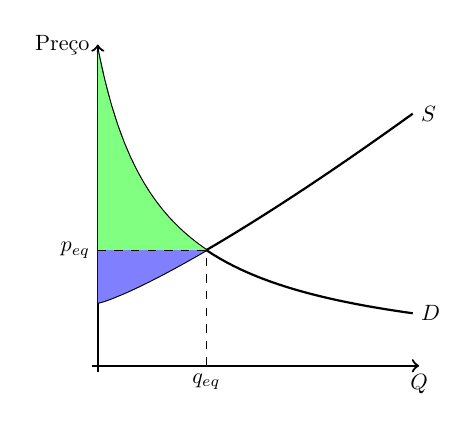
\begin{tikzpicture}[
					scale = 0.8,
					every node/.style = {scale = 0.8},
					declare function = {
						s(\x) = 1+(\x/2)^(3/2.5);
						d(\x) = 5/(\x+1);
					}
					]

					\def\ea{0.75}
					\def\eb{2.80397}
					\def\eq{1.72301}

					\draw[thick,->] (-0.1,0) -- (5.1,0)node[below]{$Q$};
					\draw[thick,->] (0,-0.1) -- (0,5.1)node[left]{Pre\c co};

					\draw[thick,samples=50,domain=0:5,variable=\x] plot (\x,{d(\x)}) node[right]{$D$};
					\draw[thick,samples=50,domain=0:5,variable=\x] plot (\x,{s(\x)}) node[right]{$S$};
					
					\fill[green!50!white,domain=0:\eq,variable=\x] plot (\x,{d(\x)}) -- (0,{d(\eq)});
					\fill[blue!50!white,domain=0:\eq,variable=\x] plot (\x,{s(\x)}) -- (0,{s(\eq)});

					\draw[dashed] (0,{s(\eq)})node[left]{$p_{eq}$} -- (\eq,{s(\eq)}) -- (\eq,0)node[below]{$q_{eq}$};

				\end{tikzpicture}
			\end{center}
		\end{column}
		\begin{column}{0.45\textwidth}
			\begin{center}
				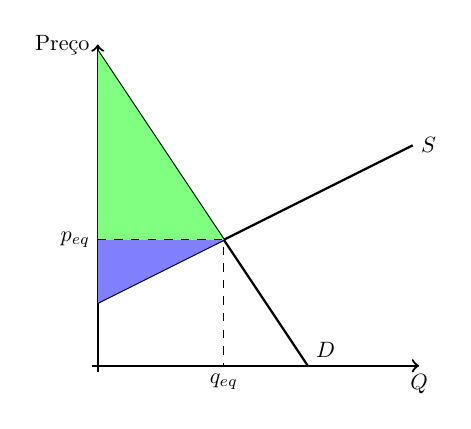
\begin{tikzpicture}[
					scale = 0.8,
					every node/.style = {scale = 0.8},
					declare function = {
						s(\x) = 1+(\x/2);
						d(\x) = 5-(3/2)*\x;
					}
					]

					\def\eq{2}

					\draw[thick,->] (-0.1,0) -- (5.1,0)node[below]{$Q$};
					\draw[thick,->] (0,-0.1) -- (0,5.1)node[left]{Pre\c co};

					\draw[thick,domain=0:(10/3),variable=\x] plot (\x,{d(\x)}) node[above right]{$D$};
					\draw[thick,domain=0:5,variable=\x] plot (\x,{s(\x)}) node[right]{$S$};

					\fill[green!50!white,domain=0:\eq,variable=\x] plot(\x,{d(\x)}) -- (0,{d(\eq)});
					\fill[blue!50!white,domain=0:\eq,variable=\x] plot(\x,{s(\x)}) -- (0,{s(\eq)});

					\draw[dashed] (0,{s(\eq)})node[left]{$p_{eq}$} -- (\eq,{s(\eq)}) -- (\eq,0)node[below]{$q_{eq}$};

				\end{tikzpicture}
			\end{center}
		\end{column}
	\end{columns}
	{\raggedleft{Na vers\~ao linear para o mercado.\par}}
\end{frame}

\begin{frame}
	\frametitle{Excedente Econ\'omico}
	\begin{itemize}
		\setlength\itemsep{1em}
		\item O Excedente Econ\'omico \'e o somat\'orio do excedente do consumidor e do excedente do produtor e representa o valor da exist\^encia de trocas no mercado. Avalia-se nas unidades monet\'arias em que est\~ao expressos os pre\c cos.
		\item Demonstra-se que este excedente \'e m\'aximo num mercado de concorr\^encia perfeita, da\'i se designar como a forma eficiente de mercado (desde que n\~ao existam falhas de mercado)
	\end{itemize}
\end{frame}

\begin{frame}
	\frametitle{Concorr\^encia Perfeita: Escolha indiv. vs Eq. de Mercado}
	A escolha \'optima de produ\c c\~ao, para cada empresa $i$, dar-se-\'a ao longo da curva de procura que lhe \'e dirigida, $D_i$, ao n\'ivel do pre\c co de equil\'ibrio $p^*$, formado pela interac\c c\~ao do conjunto dos agentes econ\'omicos.
	\begin{center}
		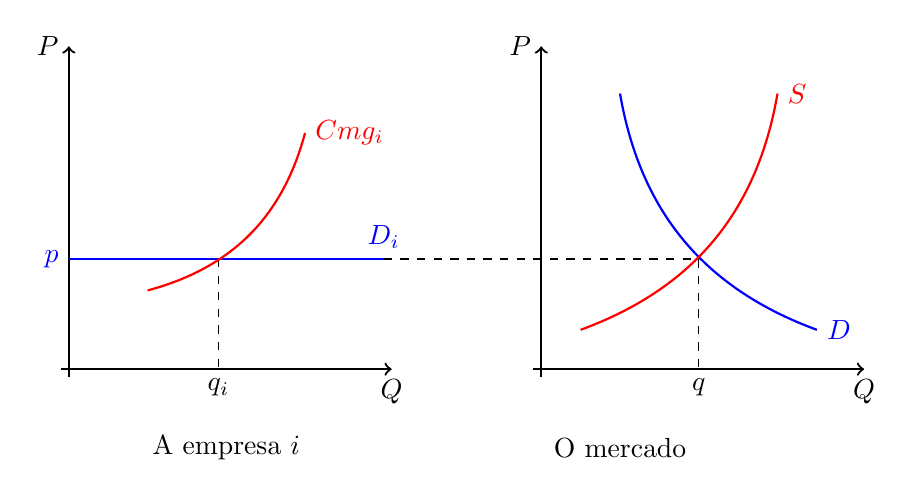
\begin{tikzpicture}[
			scale = 1,
			every node/.style = {scale = 1}
			]

			\def\p{1.4}
			\def\q{8}
			\def\qi{1.9}
			

			\draw[thick,->] (-0.1,0) -- (4.1,0) node[below]{$Q$};
			\draw[thick,->] (5.9,0) -- (10.1,0) node[below]{$Q$};

			\draw[thick,->] (0,-0.1) -- (0,4.1) node[left]{$P$};
			\draw[thick,->] (6,-0.1) -- (6,4.1) node[left]{$P$};

			\draw[thick,blue] (0,\p)node[left]{$p$} -- (4,\p)node[above]{$D_i$};
			\draw[dashed] (\qi,\p) -- (\qi,0)node[below]{$q_i$};
			\draw[dashed] (4,\p) -- (\q,\p) -- (\q,0)node[below]{$q$};

			\draw[red,thick] (1,1) to [bend right] (3,3) node[right]{$Cmg_i$};

			\draw[blue,thick] (7,3.5) to [bend right] (9.5,0.5)node[right]{$D$};
			\draw[red,thick] (6.5,0.5) to [bend right] (9,3.5)node[right]{$S$};

			\draw(2,-1) node {A empresa $i$};
			\draw(7,-1) node {O mercado};

		\end{tikzpicture}
	\end{center}
	
\end{frame}